\setcounter{secnumdepth}{2}
\chapter{Theoretical Preliminaries}
\section{Theoretical Background}
An antenna is an electrical component that acts as a transducer between a guided electrical signal and a propagating electromagnetic wave. To analyze its behavior within an electrical system, an equivalent circuit was drawn. In transmission mode, a signal source feeds the antenna, which has an impedance $Z_a$. This impedance consists of a radiation resistance $R_{ar}$, representing the power radiated into space, and a loss resistance $R_{al}$, representing ohmic losses. In reception mode, an incoming electromagnetic wave induces an open-circuit voltage $V_{oc}$ at the antenna's terminals, which then delivers a signal to the receiver's load impedance $Z_L$.


\begin{figure}[h!]
	\centering
	\begin{subfigure}[t]{0.48\textwidth}
		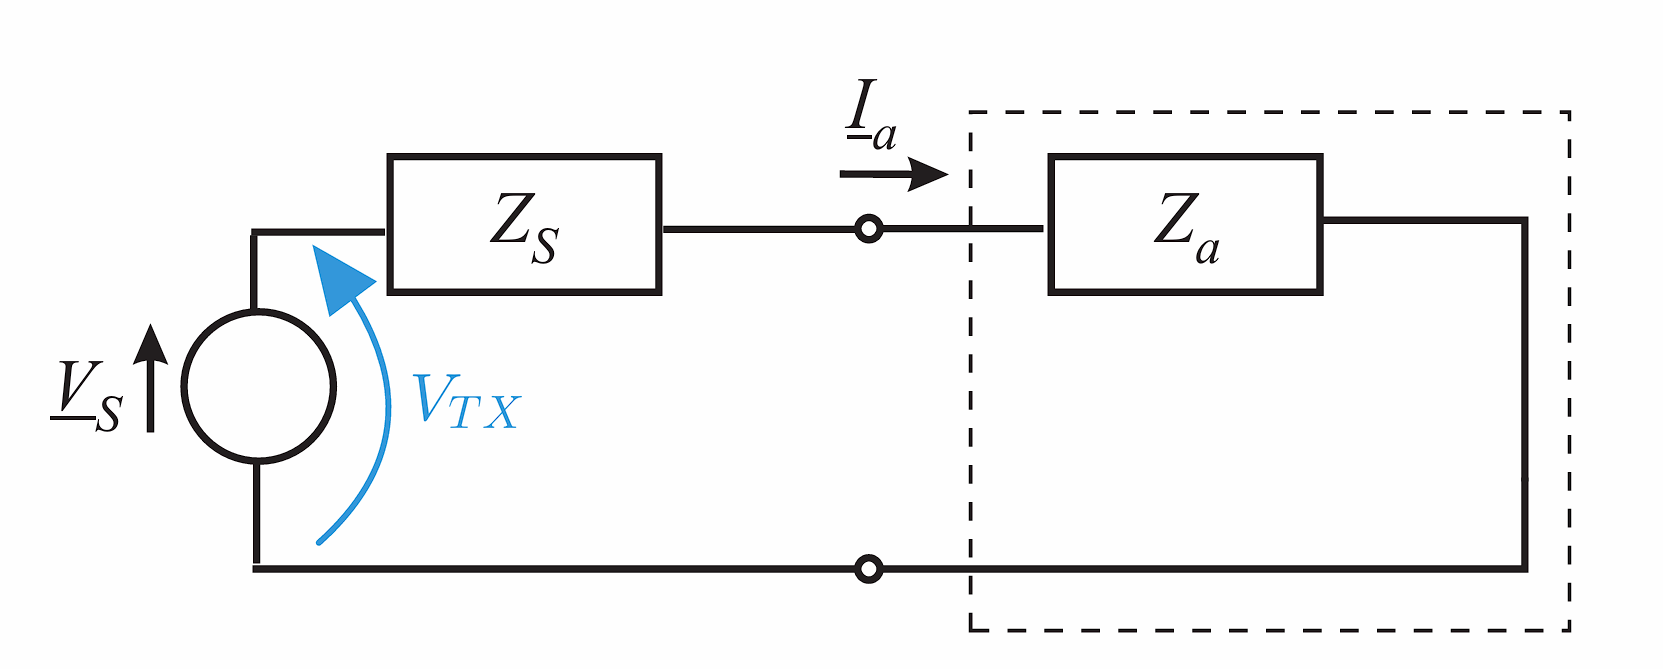
\includegraphics[width=\linewidth]{content/4-images/ant-recep.png}
		\caption{Transmit antenna equivalent circuit, showing the source voltage $V_S$, source impedance $Z_S$, transmit voltage $V_{TX}$, and antenna current $I_a$.}
		\label{fig:tx_circuit}
	\end{subfigure}
	\hfill
	\begin{subfigure}[t]{0.42\textwidth}
		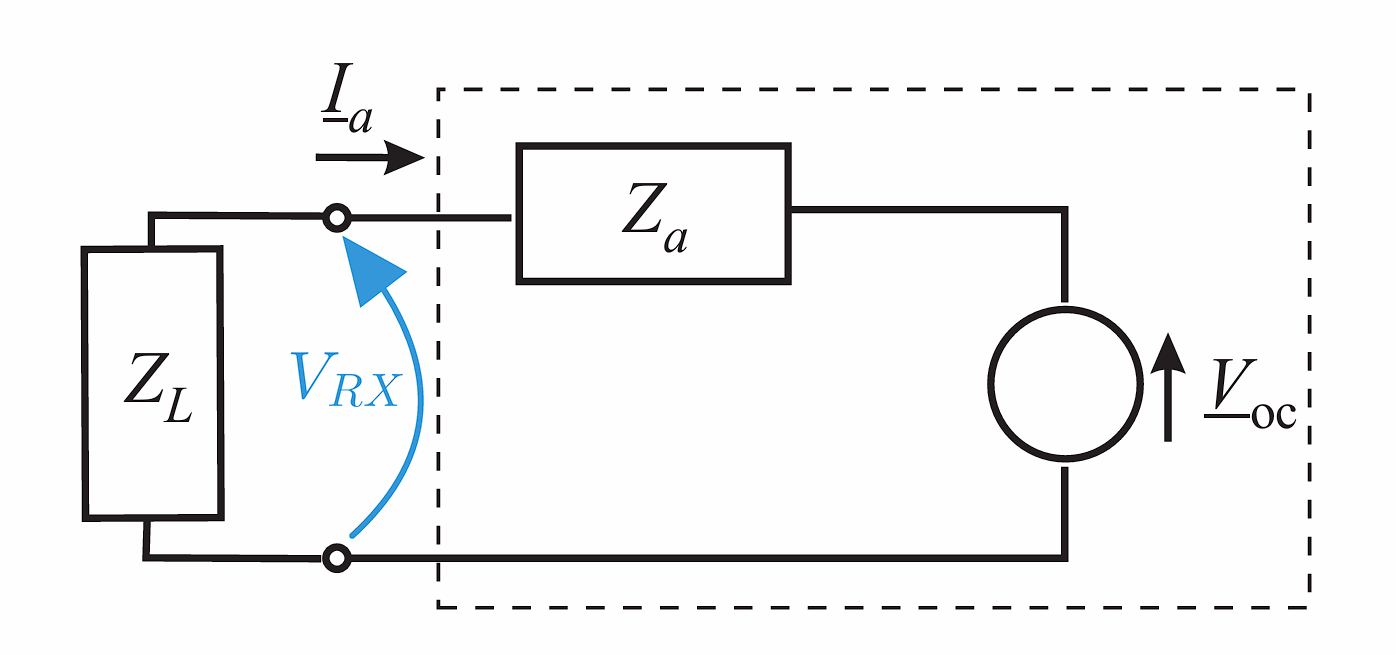
\includegraphics[width=\linewidth]{content/4-images/ant-trans.png}
		\caption{Receive antenna equivalent circuit, showing the induced open-circuit voltage $V_{oc}$, the load impedance $Z_L$, and the received voltage $V_{RX}$.}
		\label{fig:rx_circuit}
	\end{subfigure}
	\caption{Equivalent circuits for the transmit and receive antennas}
	\label{fig:equivalent_circuits}
\end{figure}

The equivalent circuits for the transmitter and receiver are drawn in Figure \ref{fig:equivalent_circuits}. In Figure \ref{fig:tx_circuit}, can be seen the equivalent circuit of the transmitter. The voltage source $V_S$ with its internal impedance $Z_S$ drives the antenna, resulting in a current $I_a$ and a voltage $V_{TX}$ at the antenna's input terminals. At the receiver (Figure \ref{fig:rx_circuit}), the incoming wave induces an open-circuit voltage $V_{oc}$, which in turn produces the received voltage $V_{RX}$ across the load impedance $Z_L$.

For this project, it was considered that the electronics are perfectly matched to the antennas. This implies that for the transmitter, the source impedance is the complex conjugate of the antenna impedance:
\begin{equation}
	Z_S = Z_a^*
\end{equation}
\vspace{0.5em}
and for the receiver, the load impedance is the complex conjugate of the antenna impedance:
\begin{equation}
	Z_L = Z_a^*
\end{equation}
\vspace{0.5em}
This consideration ensures maximum power transfer.

\subsection{Antenna Effective Height}
\begin{figure}[H]
	\centering
	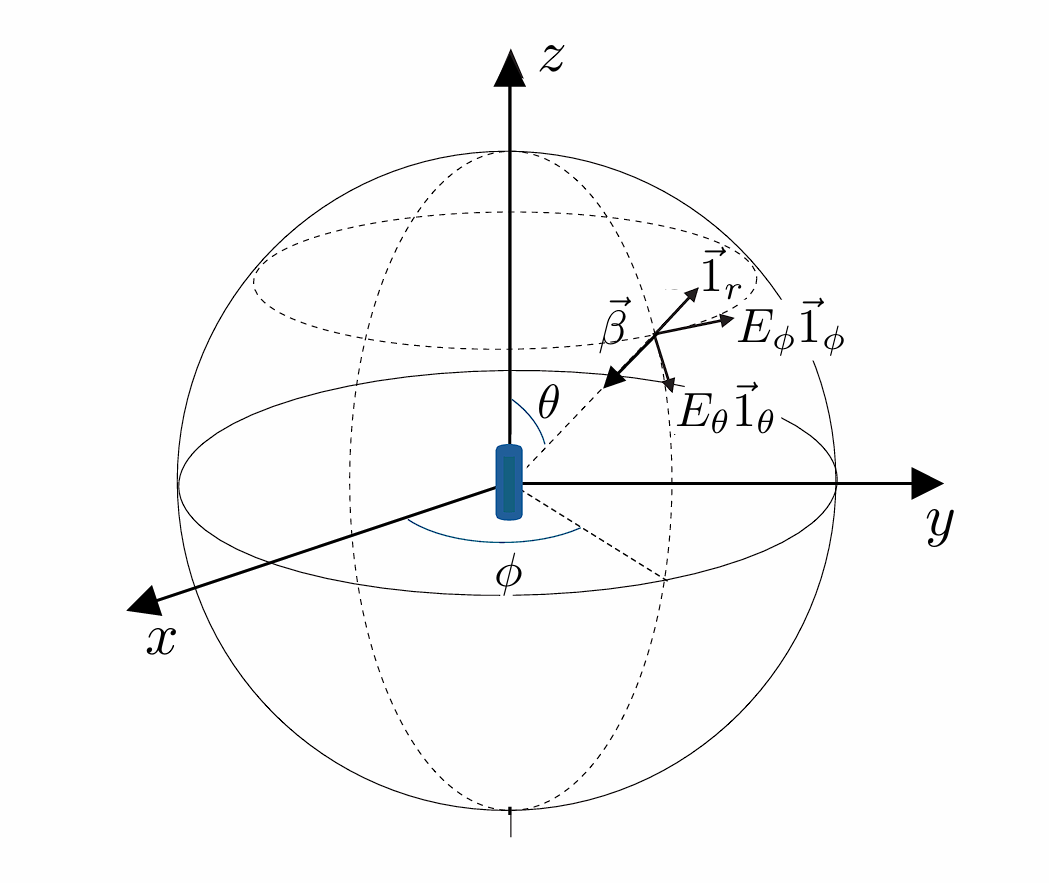
\includegraphics[width=0.5\linewidth]{content/4-images/axes.png}
	\caption{Illustration of the vertical dipole antenna and coordinate axes.}
	\label{fig:axes}
\end{figure}

The effective height $\vec{h}_e$ of an antenna links the circuit domain to the electromagnetic wave domain. It is derived from the current distribution $\vec{J}(\vec{r}\hspace{0.2em}')$ on the antenna when transmitting with an input current $\underline{I}_a$:
\begin{equation}
	\vec{h}_e(\theta, \phi) = \frac{1}{\underline{I}_a} \int_{\mathcal{D}} \vec{J}(\vec{r}\hspace{0.2em}') e^{j\beta(\vec{r}\hspace{0.2em}' \cdot \vec{1}_r)} dV'
	\label{eq:he_general}
\end{equation}
\vspace{0.5em}
where $\mathcal{D}$ is the volume of the antenna, $\vec{1}_r$ is the unit vector in the direction of radiation $(\theta, \phi)$, and $\beta$ is the wavenumber:
\begin{equation}
	\beta = \frac{2\pi}{\lambda}
\end{equation}

For a thin, vertical half-wave dipole antenna of length $L=\frac{\lambda}{2}$ oriented along the z-axis and centered at the origin (Figure \ref{fig:axes}), the current flows only in the z-direction. The current distribution is given by:
\begin{equation}
	\vec{J}(\vec{r}\hspace{0.2em}') = \underline{I}_a \cos(\beta z') \delta(x') \delta(y') \vec{1}_z, \quad \text{for } -\frac{\lambda}{4} \le z' \le \frac{\lambda}{4}
\end{equation}
\vspace{0.5em}
where $\delta(x')$ and $\delta(y')$ are Dirac's deltas.

The volume integral reduces to a line integral along the z-axis. The dot product in the exponent simplifies to:
\begin{equation}
	\vec{r}\hspace{0.2em}' \cdot \vec{1}_r = z' \cos\theta
\end{equation}
\vspace{0.5em}
Substituting this into Equation \ref{eq:he_general} gives:
\begin{equation}
	\vec{h}_e(\theta, \phi) = \left( \int_{-\frac{\lambda}{4}}^{\frac{\lambda}{4}} \cos(\beta z') e^{j\beta z' \cos\theta} dz' \right) \vec{1}_z
	\label{eq:he_integral_form}
\end{equation}
\vspace{0.5em}
The integral in Equation \ref{eq:he_integral_form} is solved using Euler's formula:
\begin{equation}
	\cos(\beta z') = \frac{1}{2}(e^{j\beta z'} + e^{-j\beta z'})
\end{equation}
\begin{align}
	\int_{-\frac{\lambda}{4}}^{\frac{\lambda}{4}} \cos(\beta z') e^{j\beta z' \cos\theta} dz' &= \frac{1}{2} \int_{-\frac{\lambda}{4}}^{\frac{\lambda}{4}} \left( e^{j\beta z'(1+\cos\theta)} + e^{j\beta z'(\cos\theta-1)} \right) dz' \\[\jot]
	&= \frac{1}{2j\beta} \left[ \frac{e^{j\beta z'(1+\cos\theta)}}{1+\cos\theta} + \frac{e^{j\beta z'(\cos\theta-1)}}{\cos\theta-1} \right]_{-\frac{\lambda}{4}}^{\frac{\lambda}{4}}
\end{align}
\vspace{1em}
With $\beta = \frac{2\pi}{\lambda}$, the term $\frac{\beta\lambda}{4}$ simplifies to $\frac{\pi}{2}$. Evaluating at the limits yields:
\vspace{1em}
\begin{align}
	&= \frac{1}{2j\beta} \left[ \frac{e^{j\frac{\pi}{2}(1+\cos\theta)} - e^{-j\frac{\pi}{2}(1+\cos\theta)}}{1+\cos\theta} - \frac{e^{j\frac{\pi}{2}(1-\cos\theta)} - e^{-j\frac{\pi}{2}(1-\cos\theta)}}{1-\cos\theta} \right]
\end{align}

\vspace{1em}
Using the definition of sine: $\sin(x) = \frac{e^{jx}-e^{-jx}}{2j}$

\begin{align}
	&= \frac{1}{\beta} \left[ \frac{\sin\left(\frac{\pi}{2}(1+\cos\theta)\right)}{1+\cos\theta} - \frac{\sin\left(\frac{\pi}{2}(\cos\theta-1)\right)}{1-\cos\theta} \right] \\[\jot]
	&= \frac{1}{\beta} \left[ \frac{\sin(\frac{\pi}{2}+\frac{\pi}{2}\cos\theta)}{1+\cos\theta} + \frac{\sin(\frac{\pi}{2}-\frac{\pi}{2}\cos\theta)}{1-\cos\theta} \right]
\end{align}
\vspace{1em}
Applying the identities $\sin(\frac{\pi}{2}+x) = \cos(x)$ and $\sin(\frac{\pi}{2}-x) = \cos(x)$:
\vspace{1em}
\begin{align}
	&= \frac{1}{\beta} \left[ \frac{\cos(\frac{\pi}{2}\cos\theta)}{1+\cos\theta} + \frac{\cos(\frac{\pi}{2}\cos\theta)}{1-\cos\theta} \right] \\[\jot]
	&= \frac{\cos(\frac{\pi}{2}\cos\theta)}{\beta} \left[ \frac{(1-\cos\theta) + (1+\cos\theta)}{(1+\cos\theta)(1-\cos\theta)} \right] = \frac{2\cos(\frac{\pi}{2}\cos\theta)}{\beta\sin^2\theta}
\end{align}
\vspace{1em}
Substituting $\beta=\frac{2\pi}{\lambda}$, the final result of the integral is:
\begin{equation}
	\frac{\lambda}{\pi} \frac{\cos(\frac{\pi}{2}\cos\theta)}{\sin^2\theta}
\end{equation}
\vspace{0.5em}
The effective height for the vertical half-wave dipole is therefore:
\begin{equation}
	\vec{h}_e(\theta, \phi) = \frac{\lambda}{\pi} \frac{\cos(\frac{\pi}{2}\cos\theta)}{\sin^2\theta} \vec{1}_z
	\label{eq:he_dipole_z}
\end{equation}
\vspace{0.5em}
This vector is oriented along the z-axis. For reception, the induced voltage depends on the component of the effective height that is transverse (perpendicular) to the direction of wave propagation, $\vec{1}_r$. This transverse component is denoted $\vec{h}_{e\perp}$. The Cartesian unit vector $\vec{1}_z$ is expressed in spherical coordinates as:
\begin{equation}
	\vec{1}_z = \cos\theta \vec{1}_r - \sin\theta \vec{1}_\theta
\end{equation}
\vspace{0.5em}
The transverse part, $\vec{h}_{e\perp}$, consists of the components in the $\vec{1}_\theta$ and $\vec{1}_\phi$ directions. Substituting the spherical representation of $\vec{1}_z$ into Equation \ref{eq:he_dipole_z} and retaining only the transverse component gives:
\begin{equation}
	\vec{h}_{e\perp}(\theta, \phi) = -\frac{\lambda}{\pi} \frac{\cos(\frac{\pi}{2}\cos\theta)}{\sin^2\theta} (\sin\theta \vec{1}_\theta) = -\frac{\lambda}{\pi} \frac{\cos(\frac{\pi}{2}\cos\theta)}{\sin\theta} \vec{1}_\theta
	\label{eq:he_perp_general}
\end{equation}
\vspace{0.5em}
This is the general expression for the transverse effective height of a vertical $\frac{\lambda}{2}$ dipole. In the horizontal plane, where $\theta = \frac{\pi}{2}$, the expression simplifies significantly. The transverse effective height in the horizontal plane is therefore:
\begin{equation}
	\boxed{\vec{h}_{e\perp}\left(\theta=\frac{\pi}{2}, \phi\right) = -\frac{\lambda}{\pi} \vec{1}_\theta}
	\label{eq:he_perp_horizontal}
\end{equation}
\vspace{0.5em}
This final expression indicates that in the horizontal plane, the antenna's effective height has a constant magnitude of $\frac{\lambda}{\pi}$, is constant for all $\phi$, and is oriented in the $\vec{1}_\theta$ direction.

\subsection{Emitted Electric Field in Free-Space}
The electric field radiated by an antenna is given by:
\begin{equation}
	\underline{\vec{E}}(\vec{r}) = -j\omega \underline{I}_a \frac{\mu_0}{4\pi} \frac{e^{-j\beta r}}{r} \vec{h}_{e\perp}(\theta, \phi)
\end{equation}
\vspace{0.5em}
Substituting the transverse effective height for the horizontal plane (Equation \ref{eq:he_perp_horizontal}) into the general expression gives:
\begin{equation}
	\underline{\vec{E}}(r, \pi/2, \phi) = -j\omega \underline{I}_a \frac{\mu_0}{4\pi} \frac{e^{-j\beta r}}{r} \left(-\frac{\lambda}{\pi} \vec{1}_\theta\right) = j \underline{I}_a \frac{\omega \mu_0 \lambda}{4\pi^2} \frac{e^{-j\beta r}}{r} \vec{1}_\theta
\end{equation}
\vspace{0.5em}
Expressing this field in terms of circuit parameters involves the substitutions $\omega = 2\pi f_c$, $\lambda = \frac{c}{f_c}$, $\mu_0 = \frac{Z_0}{c}$, and propagation delay $\tau = \frac{r}{c}$. The exponential term becomes:
\begin{equation}
	e^{-j\beta r} = e^{-j\frac{2\pi}{\lambda}c\tau} = e^{-j2\pi f_c \tau}
\end{equation}
\vspace{0.5em}
The electric field is then:
\begin{equation}
	\underline{\vec{E}} = j \underline{I}_a \frac{(2\pi f_c) (\frac{Z_0}{c}) (\frac{c}{f_c})}{4\pi^2} \frac{e^{-j2\pi f_c \tau}}{c\tau} \vec{1}_\theta = j \underline{I}_a \frac{Z_0}{2\pi c\tau} e^{-j2\pi f_c \tau} \vec{1}_\theta
\end{equation}
\vspace{0.5em}
A half-wave dipole at its resonant frequency has an almost purely real impedance, meaning its reactance is negligible ($X_a \approx 0$), so $Z_a = R_a + jX_a \approx R_a$. Under the perfect matching condition ($Z_S = Z_a^*$), the total impedance in the transmitter circuit is $Z_S + Z_a \approx Z_a^* + Z_a \approx 2R_a$. The antenna current is then related to the transmit voltage by:
\begin{equation}
	\underline{I}_a = \frac{\underline{V}_{TX}}{2R_a}
\end{equation}
\vspace{0.5em}
Substituting this for $\underline{I}_a$:
\begin{equation}
	\boxed{\underline{\vec{E}} = j \frac{Z_0}{4\pi R_a c\tau} \underline{V}_{TX} e^{-j2\pi f_c \tau} \vec{1}_\theta}
	\label{eq:E_field_final}
\end{equation}

\subsection{Received Voltage in Free-Space}
The open-circuit voltage $\underline{V}_{oc}$ induced at the terminals of a receiving antenna is given by the dot product of its effective height and the incident electric field:
\begin{equation}
	\underline{V}_{oc} = -\vec{h}_{e\perp}^{RX} \cdot \underline{\vec{E}}
\end{equation}
\vspace{0.5em}
The receiving antenna is also a vertical $\frac{\lambda}{2}$ dipole, so its transverse effective height in the horizontal plane is given by Equation \ref{eq:he_perp_horizontal}. The incident electric field is given by Eq. \ref{eq:E_field_final}. The dot product is:
\vspace{1em}
\begin{align}
	\underline{V}_{oc} &= -\left(-\frac{\lambda}{\pi} \vec{1}_\theta\right) \cdot \left(j \frac{Z_0}{4\pi R_a c\tau} \underline{V}_{TX} e^{-j2\pi f_c \tau} \vec{1}_\theta\right) \\[\jot]
	&= j \frac{\lambda Z_0}{4\pi^2 R_a c\tau} \underline{V}_{TX} e^{-j2\pi f_c \tau}
\end{align}
\vspace{1em}
The voltage $\underline{V}_{RX}$ across the receiver load $Z_L$ is found using a voltage divider on the receiver equivalent circuit (Figure \ref{fig:rx_circuit}):
\begin{equation}
	\underline{V}_{RX} = \underline{V}_{oc} \frac{Z_L}{Z_a + Z_L}
\end{equation}
\vspace{0.5em}
With perfect matching ($Z_L = Z_a^*$) and a resonant dipole ($Z_a \approx R_a$), the total impedance in the receiver circuit is $Z_a + Z_L \approx R_a + R_a = 2R_a$. The expression for $\underline{V}_{RX}$ simplifies to:
\begin{equation}
	\underline{V}_{RX} \approx \frac{\underline{V}_{oc}}{2}
\end{equation}
\vspace{0.5em}
Substituting the expression for $\underline{V}_{oc}$ gives the final relationship between the received and transmitted voltages:
\begin{equation}
	\boxed{\underline{V}_{RX} = j \frac{\lambda Z_0}{8\pi^2 R_a c\tau} \underline{V}_{TX} e^{-j2\pi f_c \tau}}
	\label{eq:VRX_vs_VTX}
\end{equation}
